\chapter{Analysing your data}
The easiest way to use your data is by looking at the PNG images of your
spectra, these can be downloaded from the SALSA data archive at the SALSA
website. 

\section{Measure velocities}
We want to measure the velocities of the different components of each spectrum.
Now you need to inspect each spectrum, and measure the velocity of each
component. This can be done using the cursor, or you may want to zoom to read
the velocities more accurately.  

At this time, it is judicious to open a spreadsheet \footnote{If you have
MS-office on your computer, use Excel for this part of the exercise. If not,
the free office suite LibreOffice (\url{http://www.libreoffice.org}) can be
used.} into which relevant numbers can be written. 
In the first column of the table, write the Galactic longitude at which the
spectrum was taken, and in the second column the velocity that you measure for
each velocity component.  If a spectrum has multiple components, write several
lines in your Excel or OpenOffice table, like:
\begin{displaymath}
\begin{array}{lr}
50 	&-48	\\
50 	& 12	\\
50	& 25	\\
70	&-90	\\
70	&-22	\\
70	&2	\\
\end{array}
\end{displaymath}
This means that the spectrum at Galactic longitude $l=50$ has three
velocity components ($-48$, 12 and 25~km/s), and the spectrum at
longitude $l=70$ also has three components.

\subsection{Subtract a baseline to correct for the zero level}
This step is not absolutely necessary if you are interested only in measuring
velocities (as in this exercise) and not intensities.  In general, the zero
level of the measured spectrum is not exactly zero. In addition, the ``zero
level'' is sometimes not perfectly flat as a function of velocity or frequency.
Therefore, one usually subtracts a baseline (a polynomial, usually of
first-order) from the data to correct for this.  To do this you need to read
the FITS file, using any of the softwares listed on the SALSA webpage.
Please note though that although this step may make your final results
clearer, it is not necessary and you should get good results also using
only the PNG images.

\section{Make the rotation curve of the Milky Way}
Now we want to construct a rotation curve from the data points we have
gathered. In Chapter~2, we showed that if we observe gas in the tangential
point, the distance from the center of the Milky Way to the cloud can be found.
The velocity of the cloud could also be calculated. In this section we are only
interested in the maximum velocity in each spectrum, which corresponds to
hydrogen at the tangential point.

To implement this analysis in a spreadsheet, 
\begin{itemize}

\item write two columns with
$l$ and $V_{r,max}$. 
 
We will now need to use the values $R_0$ and
$V_0$ in the calculations. It is possible to write them directly into
the formulae given in the previous section, 
but it is better to define them as constants in the
current file. 

\item Write the values of $R_0$
and $V_0$ into two cells. Go to {\tt Insert} $\Rightarrow$ {\tt Names}
$\Rightarrow$ {\tt Define}. A box appears. Write {\tt R0} in the top
field. Put the cursor in the lower field and then click in the cell
containing the value of $R_0$. The name of the cell appears in the
box. Click add, then repeat the process for $V_0$.

You can now use {\tt R0} and {\tt V0} directly in the formulae. 

\item Now we want to calculate $R$ and $V$, using eq.~\ref{eq-rv}. 
Start a third column where $R$ will be written. 
Click in the first cell and enter the formula 

{\tt =R0*SIN(A4*PI()/180)}

where we have converted the degrees to radians and assumed that the
first $l$ is in cell A4. Complete the row by marking the cell with the
formula and drag in the lower right corner. You have now calculated $R$
for all the clouds at the tangent point.

\item In the next column, write the formula 

{\tt =B4+V0*SIN(A4*PI()/180)}

(eq.~\ref{eq-rv}), where we assumed that the velocity is in cell B4. Finish by completing
the column for all longitudes.  

\end{itemize}

Now, you have the velocities and distances to the hydrogen gas cloud at several tangential 
points. We want to plot them in a diagram.  

\begin{itemize}

\item Begin by selecting
the entire third and fourth column. Chose {\tt Insert} $\Rightarrow$
{\tt Chart} and choose {\tt xy-chart} without lines between the points. Then
click {\tt Create} and the chart appears on the spreadsheet.

\item You can now adjust the size of the diagram; by right-clicking on it 
you can set labels on the axis and a title.

\end{itemize}

The plot should show an almost constant rotation curve. 

\begin{figure}[t]
\begin{center}
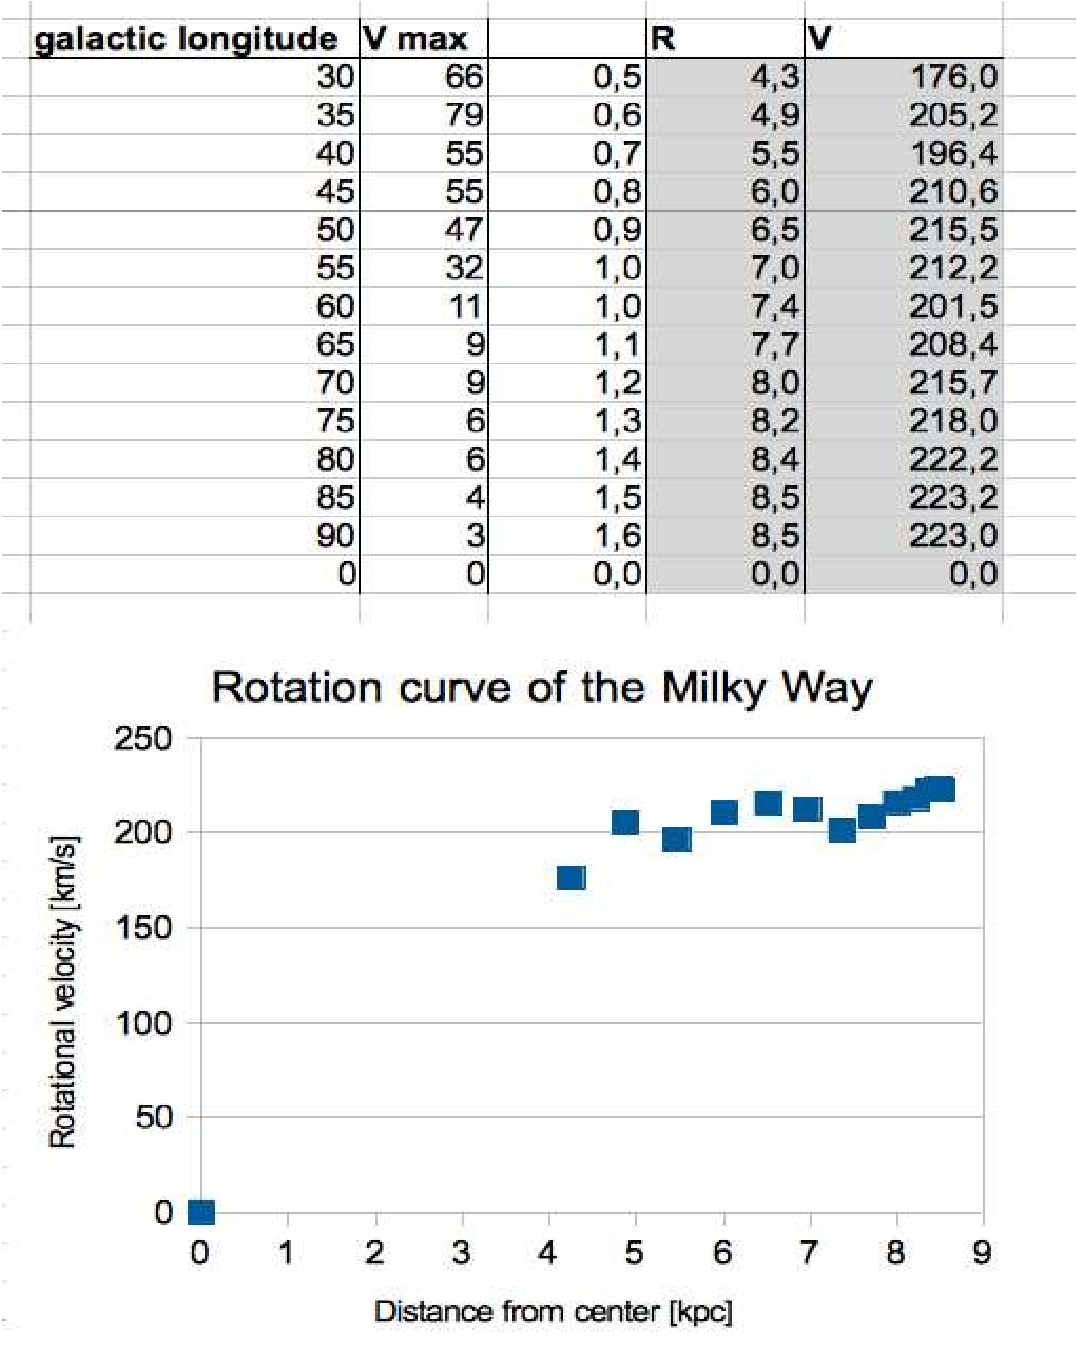
\includegraphics[width=10cm]{../figures/openofficerotation.pdf}
\caption{Example of a table and a rotation curve calculated using OpenOffice.}
\label{spread}
\end{center}
\end{figure}

\subsection{Map of the Milky Way}

In this exercise we will use all velocities measured in the spectra. We want
to construct a map of the hydrogen gas in the Galaxy. We follow the
procedure outlined in section~\ref{secmap}.  

\begin{itemize} 

\item
Make sure that you have written velocities with corresponding Galactic
longitudes in two separate columns.  

\item First, we want to calculate
$R$, the distance to the center of the Galaxy (eq.~\ref{Req}). 
Enter the formula for $R$. You will
have to use the functions

\begin{itemize} 
\item {\tt SIN()} 
\item {\tt PI()}
\end{itemize} 

\item Calculate $r$, the distance from us to the
cloud. Look at equation~\ref{rpm}. Since this is a second degree
equation in $r$ you will get two solutions. Calculate $r_{\pm}$ and
write them into two new columns. You will need the functions

\begin{itemize} 

\item{ {\tt POWER()} (that is, if you want cell $\tt A4^2$,
write {\tt POWER(A4,2)}}

\item {{\tt SIN()} (remember to convert to radians) }

\item {\tt COS()}

\item {\tt PI()}

\item{\tt SQRT()}

\end{itemize} 

If you read section~\ref{secmap} carefully, you noticed that in the
first and fourth quadrants the solution to this equation is not
unique, and thus we may have two positive solutions. Additional
measurements are needed to confirm which is the correct answer. Also, 
two negative solutions may occur, then you must discard this data
point.

Now we are almost there! We have to calculate the xy-coordinates for the data points. 
The following formulae should be familiar to you.

\begin{equation}
\left\{ 
\begin{array}{l}
x=r \cos \theta \\
y=r \sin \theta \\
\end{array}
\right.
\label{polar}
\end{equation} 

To convert to $xy$-coordinates we need to think about how angles are
defined in our coordinate system. Look at figure~\ref{coord}. The
definition of $l$ (Galactic) and $\theta$ (polar) are clearly
different. We find that $\theta=270^\circ +l$, which can be rewritten as
$\theta=l-90^\circ$.


\begin{figure}[ht]
\begin{center}
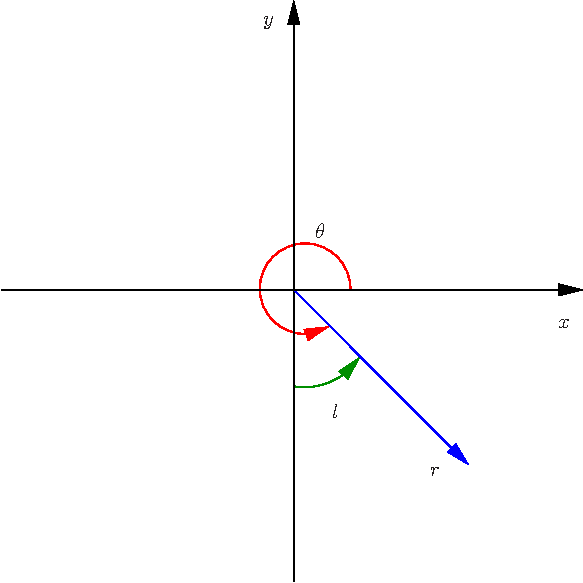
\includegraphics[width=5cm]{../figures/coordinate.pdf}
\caption{Illustration of polar ($r$,$\theta$) versus Galactic
  ($r$,$l$) coordinates.}
\label{coord}
\end{center}
\end{figure}


\item Now, calculate $x$ and $y$ by using equation~\ref{polar}.  If
  you want the origin (0,0) to be in the Galactic center, add $R_0$ to
  the $y$-coordinate.


\item Select the cells containing the $xy$-coordinates and insert a
  chart.  You will now be able to see where the hydrogen is in the
  Galaxy, and the graph should show hints of spiral arms around the
  Galactic center.

\end{itemize}

\begin{figure}[ht]
\begin{center}
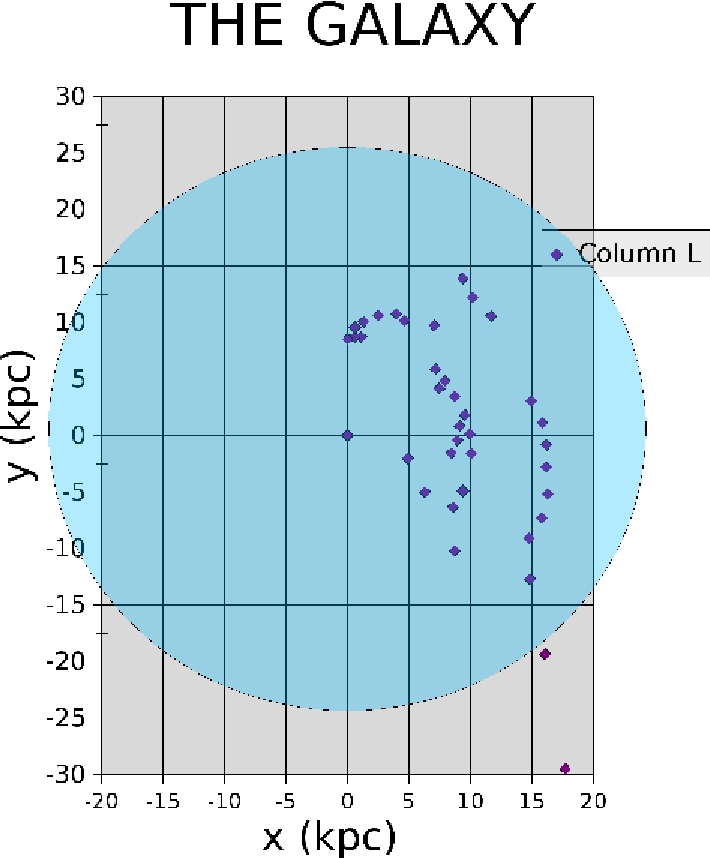
\includegraphics[width=7cm]{../figures/galaxopenoffice1.pdf}
\caption{Snapshot of the $xy$-chart in OpenOffice.  You can clearly
  see the spiral arms in the Galaxy.  The blue circle represents the
  area of the Galaxy, which has diameter of 50~kpc.}
\label{galax}
\end{center}
\end{figure}
